\documentclass[12pt]{scrartcl}

\usepackage[utf8]{inputenc}
\renewcommand*\familydefault{\sfdefault}
\usepackage[T1]{fontenc}
\usepackage[british]{babel}
\usepackage{lmodern}
\usepackage{graphicx}
\usepackage[pdftex,hyperref,dvipsnames,table]{xcolor}
\usepackage{listings}
\usepackage[a4paper,lmargin={2cm},rmargin={2cm},tmargin={3.5cm},bmargin = {2.5cm},headheight = {4cm}]{geometry}
\usepackage{amsmath,amssymb,amstext,amsthm}
\usepackage{stmaryrd}
\usepackage[lined,algonl,boxed]{algorithm2e}
\usepackage{algpseudocode}
\usepackage{tikz}
\usepackage[hidelinks]{hyperref}
\usepackage{url}
\usepackage[inline]{enumitem}
\usepackage[headsepline]{scrlayer-scrpage} 
\pagestyle{scrheadings} 
\usetikzlibrary{automata,positioning}
\usepackage{pgfplots}
\usepackage{amsfonts}
\usepackage{pdfpages}
\usepackage{listings}
\usepackage{float}
\usepackage{tcolorbox}
\usepackage{multirow}

%%%
% Enables inclusion of SVG graphics - 1:1 approach
% This is NOT the approach of http://www.ctan.org/tex-archive/info/svg-inkscape,
% which allows text in SVG to be typeset using LaTeX
% We just include the SVG as is
\usepackage{epstopdf}
\epstopdfDeclareGraphicsRule{.svg}{pdf}{.pdf}{%
  inkscape -z -D --file=#1 --export-pdf=\OutputFile
}
%
%%%



\ihead{University of Stuttgart, ITI}
%\chead{\today}
\ohead{EduSoC v1.0}

\title{EduSoC v1.0 Documentation}
\subtitle{Minimalistic RISC-V-oriented SoC for educational purposes}
\author{Alexander Kharitonov\\University of Stuttgart, ITI}

\newcommand{\paren}[1]{\left(#1\right)}
\newcommand{\abs}[1]{\left|#1\right|}
\newcommand{\angles}[1]{\left\langle#1\right\rangle}
\newcommand{\squares}[1]{\left[#1\right]}
\newcommand{\ceil}[1]{\left\lceil#1\right\rceil}
\newcommand{\floor}[1]{\left\lfloor#1\right\rfloor}
\newcommand{\set}[1]{\left\{#1\right\}}
\newcommand{\ttt}[1]{\texttt{#1}}

\setlength{\parindent}{0em}
\setlength{\parskip}{.7em}
\setlength{\intextsep}{0em}


\begin{document}

\maketitle

\section*{Overview}\label{sec:overview}
EduSoC (Educational System on Chip) is an FPGA-based, RISC-V-oriented system-on-chip infrastructure.
It is designed for educational purposes, offering minimal complexity and consisting of a small set of essential modules and peripherals:
\begin{itemize}
    \item Clock and reset signal generation
    \item Boot ROM (size and speed configurable)
    \item Block RAM (size and speed configurable)
    \item SoC controller with interrupt engine supporting up to 32 interrupts
    \item GPIO module with change notification interrupt, supporting up to 512 GPIO pins
    \item Timer module with up to 16 independent timers with configurable periods and interrupts
    \item PWM module with up to 16 independent pulse width modulated outputs
    \item VGA controller with 8-bit color framebuffer (size and speed configurable)
    \item Serial UART bridge for external memory programming and SoC/peripheral control
    \item Crossbar bus interconnect
\end{itemize}
In its default configuration, EduSoC is intended for use with a Digilent Arty S7 board and offers a Verilog-compatible module for use with this board (\ttt{edusoc\_basic}, see Appendix \ref{sec:basic}). However, EduSoC can be configured for any hardware platform, and more peripherals can be added to EduSoC with relative ease.

EduSoC does not target or contain any specific RISC-V core. A simple core interface is provided.

\newpage
\tableofcontents
\listoffigures
\listoftables
\newpage

\section{System Structure}\label{sec:structure}
\begin{figure}[H]
    \centering
    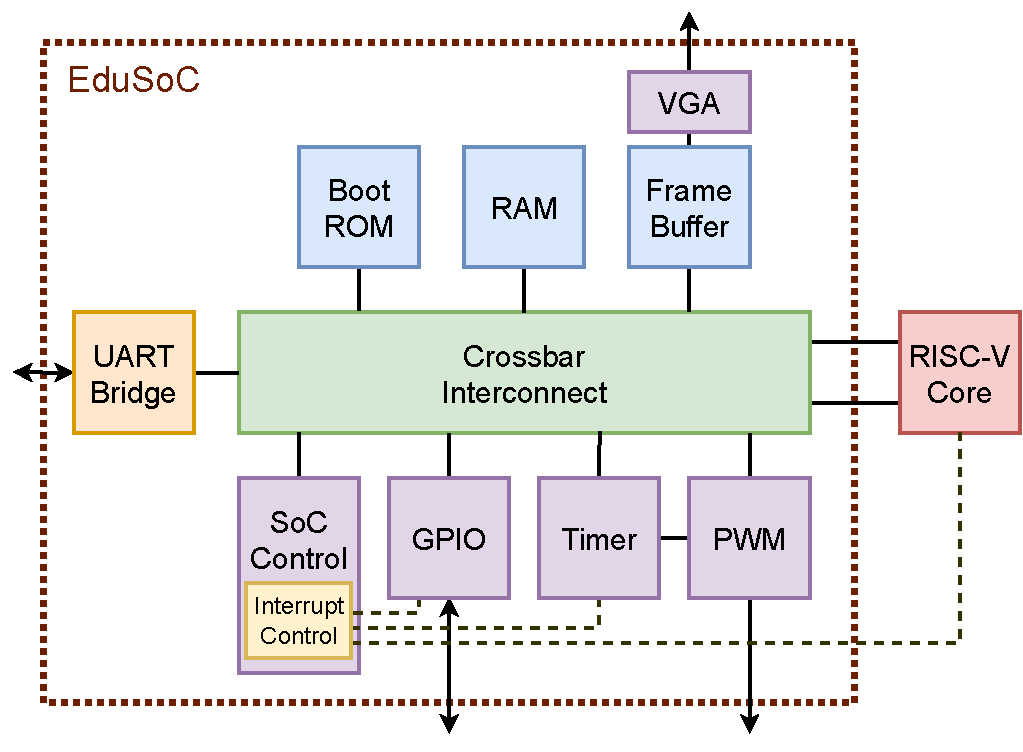
\includegraphics[width=\textwidth]{graphics/EduSoC Block Diagram.pdf}
    \vspace{-2em}
    \caption{System Block Diagram}
    \label{fig:block_diagram}
\end{figure}
EduSoC provides all components within the dotted frame. 

At its center, the crossbar interconnect serves as a bus connection between all system components.
The interconnect arbitrates three bus masters (the UART bridge and the core's data and instruction buses), where the UART bridge has priority over the other two.
The remaining SoC modules are bus slaves.

\newpage
\section{Memory Map}\label{sec:memorymap}
\begin{figure}[H]
    \centering
    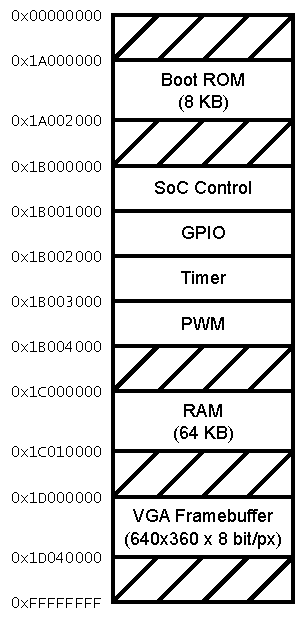
\includegraphics[height=.6\paperheight]{graphics/EduSoC Memory Map.pdf}
    \caption{Default Memory Map}
    \label{fig:memory_map}
\end{figure}
The above memory map represents the default configuration of EduSoC, and is fully configurable (see Section \ref{sec:config}).

Hatched areas are unused. Writing to them has no effect, and reading from them produces undefined values.

\newpage
\section{Interfaces}\label{sec:interfaces}
\subsection{Memory Bus}\label{sec:membus}
The EduSoC memory bus has the following signals:\\
\begin{table}[H]
    \centering
    \begin{tabular}{|c|c|c|}\hline
        Name & Width (bits) & Direction \\\hline\hline
        \ttt{addr} & 32 & Master $\Rightarrow$ Slave \\
        \ttt{read\_data} & 32 & Slave $\Rightarrow$ Master \\
        \ttt{write\_data} & 32 & Master $\Rightarrow$ Slave \\
        \ttt{write\_en} & 1 & Master $\Rightarrow$ Slave \\
        \ttt{byte\_en} & 4 & Master $\Rightarrow$ Slave \\
        \ttt{req} & 1 & Master $\Rightarrow$ Slave \\
        \ttt{valid} & 1 & Slave $\Rightarrow$ Master \\\hline
    \end{tabular}
    \caption{Memory Bus Signals}
    \label{tab:membus_signals}
\end{table}
\begin{itemize}
    \item \ttt{addr}: Requested byte address in the memory space. On the SoC level, only 4-byte-aligned requests are supported, so the lowest two address bits are ignored.
    \item \ttt{read\_data}: Data read from the requested address. Only valid when \ttt{valid} = 1 (see below). Value is not defined for write requests.
    \item \ttt{write\_data}: Data to be written to the requested address. Ignored for read requests.
    \item \ttt{write\_en}: Whether the current request is a read request (0) or a write request (1).
    \item \ttt{byte\_en}: Which of the four bytes of \ttt{write\_data} should actually be written. Each bit corresponds to one of the four bytes (1 = write, 0 = keep unchanged), with the lowest bit corresponding to the lowest byte. Ignored for read requests.
    \item \ttt{req}: Set high (1) by the master to request bus access. Once set, all master signals should be held at a constant value until the \ttt{valid} signal is 1 (see below).
    \item \ttt{valid}: Set high (1) by the slave once the master's request has been completed. For read requests, this means valid read data is available on \ttt{read\_data}, for write requests, this means the data from \ttt{write\_data} has been written to the bus.
\end{itemize}
Once \ttt{valid} is asserted high (1), the request is considered complete and potential read data stays available until the request is terminated, either by resetting \ttt{req} to 0, or by changing \ttt{addr} or \ttt{write\_en} (which constitutes a new request).

This also means that multiple consecutive requests may be made by keeping \ttt{req} = 1 and changing \ttt{addr} and/or \ttt{write\_en} once the previous request is complete.

The following are example waveforms for read and write requests to the memory bus.
\begin{figure}[h!]
    \centering
    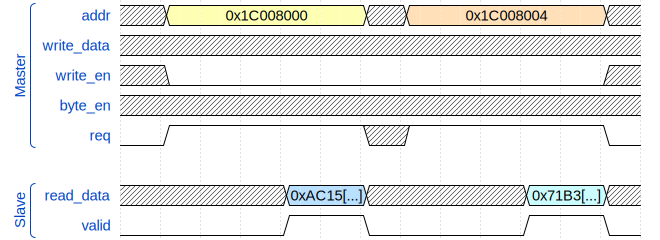
\includegraphics[width=\textwidth]{graphics/EduSoC_Bus_Read.svg}
    \vspace{-1em}
    \caption{Example Read Waveform}
    \label{fig:read_waveform}
\end{figure}
\begin{figure}[h!]
    \vspace{1em}
    \centering
    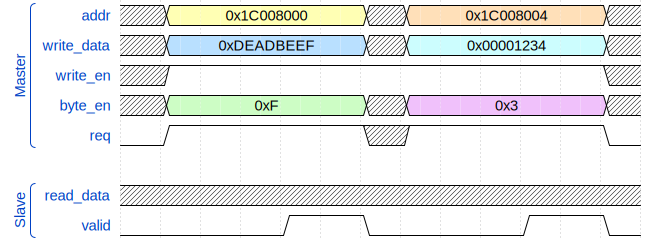
\includegraphics[width=\textwidth]{graphics/EduSoC_Bus_Write.svg}
    \vspace{-1em}
    \caption{Example Write Waveform}
    \label{fig:write_waveform}
\end{figure}

\subsection{Interrupt Bus}\label{sec:intbus}
The EduSoC interrupt bus has the following signals:\\
\begin{table}[H]
    \centering
    \begin{tabular}{|c|c|c|}\hline
        Name & Width (bits) & Direction \\\hline\hline
        \ttt{irq} & 1 & Generator $\Rightarrow$ Handler \\
        \ttt{irq\_id} & 5 & Generator $\Rightarrow$ Handler \\
        \ttt{irq\_ack} & 1 & Handler $\Rightarrow$ Generator \\
        \ttt{irq\_ack\_id} & 5 & Handler $\Rightarrow$ Generator \\\hline
    \end{tabular}
    \caption{Interrupt Bus Signals}
    \label{tab:intbus_signals}
\end{table}
\begin{itemize}
    \item \ttt{irq}: Set high (1) by the generator when an interrupt has occurred. Held until the interrupt is is acknowledged by the handler.
    \item \ttt{irq\_id}: When \ttt{irq} = 1, conveys the ID of the interrupt to be handled (see Section \ref{sec:interrupts}).
    \item \ttt{irq\_ack}: Set high (1) by the handler to signal that the currently asserted interrupt has been acknowledged and is being handled.
    \item \ttt{irq\_ack\_id}: When \ttt{irq\_ack} = 1, conveys the ID of the interrupt that is being acknowledged.
\end{itemize}

\subsection{SoC Interface}\label{sec:socinterface}
The SoC interface, consisting of the I/O interface and the CPU core interface, has the following signals and buses:\\
\begin{table}[H]
    \centering
    \begin{tabular}{|c|c|c|}\hline
        Name & Type or width (bits) & Direction \\\hline\hline
        \ttt{ext\_clk} & 1 & SoC input \\
        \ttt{ext\_resn} & 1 & SoC input \\
        \ttt{vga\_hsync} & 1 & SoC output \\
        \ttt{vga\_vsync} & 1 & SoC output \\
        \ttt{vga\_r} & 4 & SoC output \\
        \ttt{vga\_g} & 4 & SoC output \\
        \ttt{vga\_b} & 4 & SoC output \\
        \ttt{uart\_rx} & 1 & SoC input \\
        \ttt{uart\_tx} & 1 & SoC output \\
        \ttt{gpio\_in} & $N$ & SoC input \\
        \ttt{gpio\_out} & $N$ & SoC output \\
        \ttt{gpio\_drive} & $N$ & SoC output \\
        \ttt{pwm} & $M$ & SoC output \\
        \ttt{core\_clk} & 1 & SoC output \\
        \ttt{core\_res} & 1 & SoC output \\
        \ttt{control\_flags} & 16 & SoC output \\
        \ttt{instr\_bus} & Memory Bus & SoC is slave \\
        \ttt{data\_bus} & Memory Bus & SoC is slave \\
        \ttt{core\_int\_triggers} & 16 & SoC input \\
        \ttt{int\_bus} & Interrupt Bus & SoC is generator \\\hline
    \end{tabular}
    \caption{SoC Interface Signals}
    \label{tab:interface_signals}
\end{table}
The following are central control signals for the system and must be connected. In a simulation environment, they may be left open, as they are driven automatically.
\begin{itemize}
    \item \ttt{ext\_clk}: Externally supplied clock signal. Must be driven by a 100 MHz clock.
    \item \ttt{ext\_resn}: External reset (active low). Must be held high (1) and may optionally be asserted low (0) to reset the core and SoC.
\end{itemize}
Next is the VGA video output. For more information about these signals, see Section \ref{sec:vga}.
\begin{itemize}
    \item \ttt{vga\_hsync}: VGA horizontal sync signal.
    \item \ttt{vga\_vsync}: VGA vertical sync signal.
    \item \ttt{vga\_r}: VGA red color signal (16 levels).
    \item \ttt{vga\_g}: VGA green color signal (16 levels).
    \item \ttt{vga\_b}: VGA blue color signal (16 levels).
\end{itemize}
The following is the UART interface for external control and programming of the SoC. See Section \ref{sec:uart} for more information.
\begin{itemize}
    \item \ttt{uart\_rx}: UART receive line (to SoC).
    \item \ttt{uart\_tx}: UART transmit line (from SoC).
\end{itemize}
The following is the GPIO interface, with bit width $N = 32 \cdot \text{\#ports} \leq 512$. The three signals are designed to be combined into a single $N$-bit bidirectional I/O port. For more information, see Section \ref{sec:per_gpio}.
\begin{itemize}
    \item \ttt{gpio\_in}: GPIO input signals.
    \item \ttt{gpio\_out}: GPIO output signals.
    \item \ttt{gpio\_drive}: GPIO driver controls. If a bit is 0, that pin of the port is an input (``high impedance''), reading from the corresponding \ttt{gpio\_in} bit. If a bit is 1, that pin of the port is an output, writing to the corresponding \ttt{gpio\_out} bit.
\end{itemize}
The following is the output for the PWM modules, containing $M$ pulse width modulated signals, where $M \leq 16$ is the number of PWM modules in the SoC. See Section \ref{sec:per_pwm} for more information.
\begin{itemize}
    \item \ttt{pwm}: PWM output signals.
\end{itemize}
Finally, the following is the CPU core interface. See Sections \ref{sec:membus} and \ref{sec:intbus} for the memory and interrupt bus descriptions, respectively.
\begin{itemize}
    \item \ttt{core\_clk}: CPU core clock.
    \item \ttt{core\_res}: CPU core reset, active high. Intended as a synchronous reset, so the core should be reset on the rising edge of \ttt{core\_clk} if this signal is high (1).
    \item \ttt{control\_flags}: User definable control signals for the core. See Section \ref{sec:per_control} for more information.
    \item \ttt{instr\_bus}: CPU instruction memory bus. Intended to be used by the core to load program instructions from memory.
    \item \ttt{data\_bus}: CPU data memory bus. Intended to be used by the core to read and write memory or peripheral register values.
    \item \ttt{core\_int\_triggers}: Core interrupt triggers. If asserted high, a corresponding interrupt will be triggered. See Section \ref{sec:interrupts} for more information.
    \item \ttt{int\_bus}: CPU interrupt bus.
\end{itemize}

\section{Interrupts}\label{sec:interrupts}
EduSoC contains a simple interrupt controller to notify the core of asynchronous events. It supports up to 32 distinct interrupts, designated by interrupt IDs (0-31).

The priority order of the interrupts is fixed, where interrupts with a lower ID are forwarded to the core/handler first.

16 of these interrupts are SoC interrupts, generated by SoC modules and peripherals. The remaining 16 interrupts are core interrupts, which may be triggered by any events internal to the core.
To trigger such an interrupt, the corresponding bit in the \ttt{core\_int\_triggers} signal (see Section \ref{sec:socinterface}) must be set high (1) for at least one clock cycle. The interrupt will stay asserted until it is acknowledged by the core (i.\,e. typically handled in software).

The interrupt indices are assigned as follows:\\
\begin{table}[H]
    \centering
    \begin{tabular}{|c|c||c|c||c|c||c|c|}\hline
        ID & Source & ID & Source & ID & Source & ID & Source \\\hline\hline
        \cellcolor{blue!25}0 & \cellcolor{blue!25}Core Interrupt 0 & 8 & Reserved & 16 & Reserved & \cellcolor{blue!25}24 & \cellcolor{blue!25}Core Interrupt 8 \\
        \cellcolor{blue!25}1 & \cellcolor{blue!25}Core Interrupt 1 & 9 & Reserved & 17 & Reserved & \cellcolor{blue!25}25 & \cellcolor{blue!25}Core Interrupt 9 \\
        \cellcolor{blue!25}2 & \cellcolor{blue!25}Core Interrupt 2 & 10 & Reserved & 18 & Reserved & \cellcolor{blue!25}26 & \cellcolor{blue!25}Core Interrupt 10 \\
        \cellcolor{blue!25}3 & \cellcolor{blue!25}Core Interrupt 3 & \cellcolor{red!25}11 & \cellcolor{red!25}Timer & 19 & Reserved & \cellcolor{blue!25}27 & \cellcolor{blue!25}Core Interrupt 11 \\
        \cellcolor{blue!25}4 & \cellcolor{blue!25}Core Interrupt 4 & 12 & Reserved & 20 & Reserved & \cellcolor{blue!25}28 & \cellcolor{blue!25}Core Interrupt 12 \\
        \cellcolor{blue!25}5 & \cellcolor{blue!25}Core Interrupt 5 & 13 & Reserved & 21 & Reserved & \cellcolor{blue!25}29 & \cellcolor{blue!25}Core Interrupt 13 \\
        \cellcolor{blue!25}6 & \cellcolor{blue!25}Core Interrupt 6 & 14 & Reserved & 22 & Reserved & \cellcolor{blue!25}30 & \cellcolor{blue!25}Core Interrupt 14 \\
        \cellcolor{blue!25}7 & \cellcolor{blue!25}Core Interrupt 7 & \cellcolor{green!25}15 & \cellcolor{green!25}GPIO & 23 & Reserved & \cellcolor{blue!25}31 & \cellcolor{blue!25}Core Interrupt 15 \\\hline
    \end{tabular}
    \caption{Interrupt Mapping}
    \label{tab:interrupts}
\end{table}

The core should always acknowledge any asserted interrupt as soon as possible, even if that interrupt is not supported or not handled by the core. Otherwise, other interrupts may be missed, especially lower-priority ones.

Interrupts are only asserted to the core if they are enabled first, and they may be cleared by a special register write. See Section \ref{sec:per_control} for more information on interrupt control.

\newpage
\section{UART Bridge}\label{sec:uart}
The UART bridge allows EduSoC to be programmed and controlled externally through a UART interface.
The bridge functions as a memory bus master which is controlled by a UART protocol.

The UART data rate is 500000 Baud by default, but may be configured, see Section \ref{sec:config}.

The UART bridge only supports writing to the memory bus in units of 32 bit words. Each 32 bit (4 byte) word is transmitted in little endian byte order.
The UART protocol is as follows:\\
\begin{figure}[H]
    \centering
    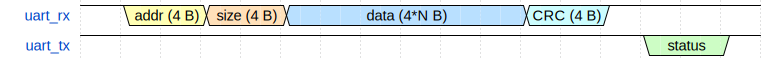
\includegraphics[width=\textwidth]{graphics/EduSoC_UART_Protocol.svg}
    \vspace{-1em}
    \caption{UART Bridge Protocol}
    \label{fig:uart_protocol}
\end{figure}
First, the starting memory address is sent (i.\,e. the address of the first word to be written). As described in Section \ref{sec:membus}, only 4-byte-aligned addresses are supported. This is followed by 4 bytes containing the size $N$ of the data to be written, \textbf{in units of 32 bit (4 byte) words} (\textit{not} bytes).

The next $N$ 32 bit words, i.\,e. $4 \cdot N$ bytes, are the actual data to be written, starting at the given address, with further words being written to the consecutively next memory addresses. Finally, the last 32 bit word is a CRC sum of the preceding data words (not including the address and size). The CRC algorithm used is CRC-32C (polynomial \ttt{0x1EDC6F41}, input and output reversed, initial value = final XOR = \ttt{0xFFFFFFFF}).

Once the bridge has received all of this data, it responds with a single byte indicating the status, which may be one of the following:\\
\begin{table}[H]
    \centering
    \begin{tabular}{|c|c|}\hline
        Value & Meaning \\\hline\hline
        0x59 & Success \\
        0x23 & CRC Mismatch \\
        0xE0 & Error \\
        Other & Unknown (error) \\\hline
    \end{tabular}
    \caption{UART Status Codes}
    \label{tab:uart_status}
\end{table}
Once a success or CRC mismatch status has been sent by the bridge, it is ready for a new transmission.
In the last two cases (error), the state of the UART bridge and the destination memory area is undefined, and the bridge may not respond to further UART transmissions. An external system reset is required to return to a known valid state.

In case of a CRC mismatch, data corruption during the transmission is possible. Note that this possibly corrupted data has been written to the destination memory area at this point, so it is recommended to retry the transmission to overwrite the corrupted data.

The EduSoC repository includes a Python script (\ttt{uart-programming/uart\_upload.py}) implementing this UART interface for the Digilent Arty S7 board. See the header comment in the script itself for more information.

\section{VGA Controller}\label{sec:vga}
EduSoC features a VGA video interface, requiring only an external DAC module for the analog color signals, for example the Digilent PmodVGA.
By default, it is configured for a 640x480 video output at 60 Hz refresh rate, where only the central 640x360 area is backed by actual pixel data.

The VGA controller is connected to the framebuffer memory, reading one byte (8 bits) of framebuffer data for each pixel, in typical scanline order, and generating all VGA interface signals from this data and its given pixel clock.
The pixel data format is RGB-332, so for each byte (= pixel), the upper three bits are the red intensity, the next three bits are the green intensity, and the lowest two bits are the blue intensity.

The framebuffer can be read and written to using the memory bus, like any other memory section, and changes to it will be visible on a connected screen immediately as soon as the changed pixels are drawn in the next frame. Note that, like any other EduSoC memory, the framebuffer contents are not affected by a system reset.

\newpage
\section{Peripherals}\label{sec:peripherals}
EduSoC contains multiple memory-mapped peripheral modules. They are accessible using the main memory bus and have registers to control their function, which are described in the following sections.

All registers in the following peripherals have four separate addresses each (differentiated by the last hexadecimal digit of the address), implementing functions for easy bit manipulations:
\begin{itemize}
    \item \ttt{0x???????0}: Main register. Allows reading the register value and writing a value directly.
    \item \ttt{0x???????4}: SET register. Reads as 0. When written: For every high (1) bit in the written value, the corresponding register bit is set high (1). Low (0) bits in the written value leave the corresponding register bits unchanged.
    \item \ttt{0x???????8}: CLEAR register. Reads as 0. When written: For every high (1) bit in the written value, the corresponding register bit is cleared (set to 0). Low (0) bits in the written value leave the corresponding register bits unchanged.
    \item \ttt{0x???????C}: INVERT register. Reads as 0. When written: For every high (1) bit in the written value, the corresponding register bit is inverted (0 $\leftrightarrow$ 1). Low (0) bits in the written value leave the corresponding register bits unchanged.
\end{itemize}
In the following register descriptions, only the main register address is given, but the SET, CLEAR, and INVERT addresses still function as described above, by using the corresponding last address digit.

The only exceptions are register bits which are read-only or may only be written in certain ways (e.\,g. clear-only bits) - the SET, CLEAR, and INVERT variants of those registers respect these restrictions, and will not perform any unsupported operations.

The register addresses given in the following register descriptions assume the default memory map described in Section \ref{sec:memorymap}.

\subsection{SoC Control}\label{sec:per_control}
The SoC control peripheral implements functions for controlling the SoC and system as a whole, as well as controlling system interrupts.

It allows software- or UART-initiated resets of the core and SoC, allows the core to be halted, and allows detailed control over interrupts (enabling/disabling interrupts globally, enabling/disabling individual interrupts, reading interrupt status, clearing individual interrupts).

Additionally, a 16 bit core control flag signal is provided (see \ttt{control\_flags} in Section \ref{sec:socinterface}). These flags may have a user-defined meaning and can also be read or written using the memory bus. Unlike most registers, these flags are \textit{not} affected by system resets, retaining their state.\\
For the bootloader code and UART programming utilities provided with EduSoC, only one of these flags (flag 0) has a meaning by default - it serves as an indicator that a program has been loaded into RAM.

This peripheral has the following registers:\\
\begin{table}[H]
    \centering
    \begin{tabular}{|c|c|l|}\hline
        Address & Name & Reset Value \\\hline\hline
        \ttt{0x1B000000} & \ttt{SOCCON\_CONTROL} & \ttt{0x00000008}\footnotemark[1] \\
        \ttt{0x1B000010} & \ttt{SOCCON\_INT\_EN} & \ttt{0x00000000} \\
        \ttt{0x1B000020} & \ttt{SOCCON\_INT\_FLAGS} & \ttt{0x00000000} \\\hline
    \end{tabular}
    \caption{SoC Control Registers}
    \label{tab:soccon_regs}
\end{table}
\footnotetext[1]{Upper 16 bits are initially 0x0000, but retain their values during further resets.}

\subsubsection{\ttt{SOCCON\_CONTROL} Register}
Address: \ttt{0x1B000000}\\
Reset value: \ttt{0x00000008}\footnotemark[1]\\
\begin{table}[H]
    \centering
    \renewcommand{\arraystretch}{1.1}
    \renewcommand{\extrarowheight}{-1.5mm}
    \begin{tabular}{|c||B|B|B|B|B|B|B|>{\arraybackslash}B|}\hline
        \rule{0pt}{12pt}Bit Range & \multicolumn{8}{c|}{Bits (highest to lowest)} \\\hline\hline
        \br{31:24} & \bd{R/W-0} & \bd{R/W-0} & \bd{R/W-0} & \bd{R/W-0} & \bd{R/W-0} & \bd{R/W-0} & \bd{R/W-0} & \bd{R/W-0} \\\cline{2-9}
        \rule{0pt}{12pt} & \multicolumn{8}{c|}{\ttt{control\_flags}[15:8]} \\\hline
        \br{23:16} & \bd{R/W-0} & \bd{R/W-0} & \bd{R/W-0} & \bd{R/W-0} & \bd{R/W-0} & \bd{R/W-0} & \bd{R/W-0} & \bd{R/W-0} \\\cline{2-9}
        \rule{0pt}{12pt} & \multicolumn{8}{c|}{\ttt{control\_flags}[7:0]} \\\hline
        \br{15:8} & \bd{U-0} & \bd{U-0} & \bd{U-0} & \bd{U-0} & \bd{U-0} & \bd{U-0} & \bd{U-0} & \bd{U-0} \\\cline{2-9}
        \rule{0pt}{12pt} & \ub & \ub & \ub & \ub & \ub & \ub & \ub & \ub \\\hline
        \br{7:0} & \bd{U-0} & \bd{U-0} & \bd{U-0} & \bd{U-0} & \bd{R/W-1} & \bd{R/W-0} & \bd{R/W-0} & \bd{R/W-0} \\\cline{2-9}
        \rule{0pt}{12pt} & \ub & \ub & \ub & \ub & \ttt{INTGEN} & \ttt{SOCRES} & \ttt{CORERES} & \ttt{COREHLT} \\\hline
        \multicolumn{9}{c}{} \\\hline
        \multicolumn{2}{|l}{\rule{0pt}{10pt}\footnotesize\textbf{Legend:}} & \multicolumn{2}{l}{\footnotesize R = Readable} & \multicolumn{2}{l}{\footnotesize W = Writable} & \multicolumn{3}{l|}{\footnotesize U = Unimplemented, read as 0} \\
        \multicolumn{2}{|l}{\rule{0pt}{10pt}\footnotesize -n = Initial Value} & \multicolumn{2}{l}{\footnotesize 1 = Set} & \multicolumn{2}{l}{\footnotesize 0 = Cleared} & \multicolumn{3}{l|}{\footnotesize x = Unknown} \\\hline
    \end{tabular}
    \renewcommand{\arraystretch}{1}
    \renewcommand{\extrarowheight}{0mm}
\end{table}
\begin{itemize}[leftmargin=18mm,labelsep=3mm,parsep=1.5mm]
    \item[\footnotesize Bit 31-16] \ttt{control\_flags}: Core control flags, see description above. Reset retains values.
    \item[\footnotesize Bit 15-4] Unimplemented: Read as 0.
    \item[\footnotesize Bit 3] \ttt{INTGEN}: Interrupt global enable.\\{\footnotesize
    0 = No interrupts will be asserted to the core, irrespective of individual interrupt enable settings.\\
    1 = Individually enabled interrupts will be asserted to the core.}
    \item[\footnotesize Bit 2] \ttt{SOCRES}: SoC software reset.\\{\footnotesize
    0 = No effect.\\
    1 = SoC will be reset on the next clock cycle (including this register/bit).}
    \item[\footnotesize Bit 1] \ttt{CORERES}: CPU core reset.\\{\footnotesize
    0 = No effect.\\
    1 = CPU core reset line is asserted high (1), leading to a reset on the next CPU core clock cycle.}
    \item[\footnotesize Bit 0] \ttt{COREHLT}: CPU core halt.\\{\footnotesize
    0 = CPU core clock is running.\\
    1 = CPU core clock is halted. Note that this also prevents synchronous core resets from occurring.}
\end{itemize}

\subsubsection{\ttt{SOCCON\_INT\_EN} Register}
Address: \ttt{0x1B000010}\\
Reset value: \ttt{0x00000000}\\
\begin{table}[H]
    \centering
    \renewcommand{\arraystretch}{1.1}
    \renewcommand{\extrarowheight}{-1.5mm}
    \begin{tabular}{|c||B|B|B|B|B|B|B|>{\arraybackslash}B|}\hline
        \rule{0pt}{12pt}Bit Range & \multicolumn{8}{c|}{Bits (highest to lowest)} \\\hline\hline
        \br{31:24} & \bd{R/W-0} & \bd{R/W-0} & \bd{R/W-0} & \bd{R/W-0} & \bd{R/W-0} & \bd{R/W-0} & \bd{R/W-0} & \bd{R/W-0} \\\cline{2-9}
        \rule{0pt}{12pt} & \multicolumn{8}{c|}{\ttt{INT\_ENABLE}[31:24]} \\\hline
        \br{23:16} & \bd{R/W-0} & \bd{R/W-0} & \bd{R/W-0} & \bd{R/W-0} & \bd{R/W-0} & \bd{R/W-0} & \bd{R/W-0} & \bd{R/W-0} \\\cline{2-9}
        \rule{0pt}{12pt} & \multicolumn{8}{c|}{\ttt{INT\_ENABLE}[23:16]} \\\hline
        \br{15:8} & \bd{R/W-0} & \bd{R/W-0} & \bd{R/W-0} & \bd{R/W-0} & \bd{R/W-0} & \bd{R/W-0} & \bd{R/W-0} & \bd{R/W-0} \\\cline{2-9}
        \rule{0pt}{12pt} & \multicolumn{8}{c|}{\ttt{INT\_ENABLE}[15:8]} \\\hline
        \br{7:0} & \bd{R/W-0} & \bd{R/W-0} & \bd{R/W-0} & \bd{R/W-0} & \bd{R/W-0} & \bd{R/W-0} & \bd{R/W-0} & \bd{R/W-0} \\\cline{2-9}
        \rule{0pt}{12pt} & \multicolumn{8}{c|}{\ttt{INT\_ENABLE}[7:0]} \\\hline
        \multicolumn{9}{c}{} \\\hline
        \multicolumn{2}{|l}{\rule{0pt}{10pt}\footnotesize\textbf{Legend:}} & \multicolumn{2}{l}{\footnotesize R = Readable} & \multicolumn{2}{l}{\footnotesize W = Writable} & \multicolumn{3}{l|}{\footnotesize U = Unimplemented, read as 0} \\
        \multicolumn{2}{|l}{\rule{0pt}{10pt}\footnotesize -n = Initial Value} & \multicolumn{2}{l}{\footnotesize 1 = Set} & \multicolumn{2}{l}{\footnotesize 0 = Cleared} & \multicolumn{3}{l|}{\footnotesize x = Unknown} \\\hline
    \end{tabular}
    \renewcommand{\arraystretch}{1}
    \renewcommand{\extrarowheight}{0mm}
\end{table}
\begin{itemize}[leftmargin=18mm,labelsep=3mm,parsep=1.5mm]
    \item[\footnotesize Bit 31-0] \ttt{INT\_ENABLE}: Individual interrupt enable.\\{\footnotesize
    0 = Interrupt with the corresponding index will not be asserted to the core.\\
    1 = Interrupt with the corresponding index will be asserted to the core whenever it occurs.}
\end{itemize}
Each bit corresponds to one interrupt ID, e.\,g. bit 0 corresponds to interrupt ID 0.

When enabling an interrupt, if it has occurred in the past (i.\,e. its flag is 1, see \ttt{SOCCON\_INT\_FLAGS}), it will immediately be asserted to the core.

\newpage
\subsubsection{\ttt{SOCCON\_INT\_FLAGS} Register}
Address: \ttt{0x1B000020}\\
Reset value: \ttt{0x00000000}\\
\begin{table}[H]
    \centering
    \renewcommand{\arraystretch}{1.1}
    \renewcommand{\extrarowheight}{-1.5mm}
    \begin{tabular}{|c||B|B|B|B|B|B|B|>{\arraybackslash}B|}\hline
        \rule{0pt}{12pt}Bit Range & \multicolumn{8}{c|}{Bits (highest to lowest)} \\\hline\hline
        \br{31:24} & \bd{R/C-0} & \bd{R/C-0} & \bd{R/C-0} & \bd{R/C-0} & \bd{R/C-0} & \bd{R/C-0} & \bd{R/C-0} & \bd{R/C-0} \\\cline{2-9}
        \rule{0pt}{12pt} & \multicolumn{8}{c|}{\ttt{INT\_FLAGS}[31:24]} \\\hline
        \br{23:16} & \bd{R/C-0} & \bd{R/C-0} & \bd{R/C-0} & \bd{R/C-0} & \bd{R/C-0} & \bd{R/C-0} & \bd{R/C-0} & \bd{R/C-0} \\\cline{2-9}
        \rule{0pt}{12pt} & \multicolumn{8}{c|}{\ttt{INT\_FLAGS}[23:16]} \\\hline
        \br{15:8} & \bd{R/C-0} & \bd{R/C-0} & \bd{R/C-0} & \bd{R/C-0} & \bd{R/C-0} & \bd{R/C-0} & \bd{R/C-0} & \bd{R/C-0} \\\cline{2-9}
        \rule{0pt}{12pt} & \multicolumn{8}{c|}{\ttt{INT\_FLAGS}[15:8]} \\\hline
        \br{7:0} & \bd{R/C-0} & \bd{R/C-0} & \bd{R/C-0} & \bd{R/C-0} & \bd{R/C-0} & \bd{R/C-0} & \bd{R/C-0} & \bd{R/C-0} \\\cline{2-9}
        \rule{0pt}{12pt} & \multicolumn{8}{c|}{\ttt{INT\_FLAGS}[7:0]} \\\hline
        \multicolumn{9}{c}{} \\\hline
        \multicolumn{2}{|l}{\rule{0pt}{10pt}\footnotesize\textbf{Legend:}} & \multicolumn{2}{l}{\footnotesize R = Readable} & \multicolumn{2}{l}{\footnotesize W = Writable} & \multicolumn{3}{l|}{\footnotesize U = Unimplemented, read as 0} \\
        \multicolumn{2}{|l}{\footnotesize C = Clearable} & \multicolumn{2}{l}{\rule{0pt}{10pt}\footnotesize -n = Initial Value} & \multicolumn{1}{l}{\footnotesize 1 = Set} & \multicolumn{2}{l}{\footnotesize 0 = Cleared} & \multicolumn{2}{l|}{\footnotesize x = Unknown} \\\hline
    \end{tabular}
    \renewcommand{\arraystretch}{1}
    \renewcommand{\extrarowheight}{0mm}
\end{table}
\begin{itemize}[leftmargin=18mm,labelsep=3mm,parsep=1.5mm]
    \item[\footnotesize Bit 31-0] \ttt{INT\_FLAGS}: Interrupt occurred flags.\\{\footnotesize
    0 = Interrupt with the corresponding index has not occurred.\\
    1 = Interrupt with the corresponding index has occurred and will be asserted to the core if it is enabled.}
\end{itemize}
Each bit corresponds to one interrupt ID, e.\,g. bit 0 corresponds to interrupt ID 0.

Flags/bits in this register may be cleared (set to 0) using memory writes, which will clear the corresponding interrupts and stop them from being asserted until they reoccur. Attempting to set bits to 1 using memory writes will have no effect.

\subsection{GPIO}\label{sec:per_gpio}

\subsection{Timer}\label{sec:per_timer}

\newpage
\subsection{PWM}\label{sec:per_pwm}
The PWM peripheral implements configurable pulse width modulated signal generation. It consists of up to 16 independent PWM modules (configurable, see Section \ref{sec:config}), where the default PWM module count is 6.

In the \ttt{edusoc\_basic} configuration, the 6 PWM modules are connected to the two RGB LEDs on the Arty S7 board, as a way to generate any desired LED colors. However, the corresponding timers and PWM modules are not automatically configured by the provided bootloader. See Appendix \ref{sec:basic} for more information.

Each PWM module depends on one timer from the timer peripheral (see Section \ref{sec:per_timer}). The PWM signal period is equal to the timer's period, and the timer must be enabled and running continuously for correct PWM signal generation. Multiple PWM modules can use the same timer.

The modulation value (pulse width) of a PWM module is controlled by its value register, which determines the absolute width of each pulse (in clock cycles). For a value of 0, the signal is constantly low (0), for a value greater than or equal to the corresponding timer period, the signal is constantly high (1).

The value register cannot be modified directly, instead, each module has a ``next value'' register which can be written to, and will be copied to the value register at the start of the following PWM/timer period.

In the following register descriptions, each type of register is only described once, even if it has multiple copies for the different PWM modules. $i$ is used as a placeholder for the module index in these cases (where the first module is $i = 0$). In register addresses, $i$ should be replaced with the hexadecimal representation of the desired module index.

This peripheral has the following registers:\\
\begin{table}[H]
    \centering
    \begin{tabular}{|c|c|l|}\hline
        Address & Name & Reset Value \\\hline\hline
        \ttt{0x1B003$i$00} & \ttt{PWM\_CONTROL\_$i$} & \ttt{0x00000000} \\
        \ttt{0x1B003$i$10} & \ttt{PWM\_VALUE\_$i$} & \ttt{0x00000000} \\
        \ttt{0x1B003$i$20} & \ttt{PWM\_NEXT\_VALUE\_$i$} & \ttt{0x00000000} \\\hline
    \end{tabular}
    \caption{PWM Registers}
    \label{tab:pwm_regs}
\end{table}

\newpage
\subsubsection{\ttt{PWM\_CONTROL\_$i$} Register}
\vspace{-3mm}
Address: \ttt{0x1B003$i$00}\hfill
Reset value: \ttt{0x00000000}\\[-1mm]
\begin{table}[H]
    \centering
    \renewcommand{\arraystretch}{1.1}
    \renewcommand{\extrarowheight}{-1.5mm}
    \begin{tabular}{|c||B|B|B|B|B|B|B|>{\arraybackslash}B|}\hline
        \rule{0pt}{12pt}Bit Range & \multicolumn{8}{c|}{Bits (highest to lowest)} \\\hline\hline
        \br{31:24} & \bd{U-0} & \bd{U-0} & \bd{U-0} & \bd{U-0} & \bd{U-0} & \bd{U-0} & \bd{U-0} & \bd{U-0} \\\cline{2-9}
        \rule{0pt}{12pt} & \ub & \ub & \ub & \ub & \ub & \ub & \ub & \ub \\\hline
        \br{23:16} & \bd{U-0} & \bd{U-0} & \bd{U-0} & \bd{U-0} & \bd{U-0} & \bd{U-0} & \bd{U-0} & \bd{U-0} \\\cline{2-9}
        \rule{0pt}{12pt} & \ub & \ub & \ub & \ub & \ub & \ub & \ub & \ub \\\hline
        \br{15:8} & \bd{U-0} & \bd{U-0} & \bd{U-0} & \bd{U-0} & \bd{U-0} & \bd{U-0} & \bd{U-0} & \bd{R/W-0} \\\cline{2-9}
        \rule{0pt}{12pt} & \ub & \ub & \ub & \ub & \ub & \ub & \ub & \ttt{ENABLE} \\\hline
        \br{7:0} & \bd{U-0} & \bd{U-0} & \bd{U-0} & \bd{U-0} & \bd{R/W-0} & \bd{R/W-0} & \bd{R/W-0} & \bd{R/W-0} \\\cline{2-9}
        \rule{0pt}{12pt} & \ub & \ub & \ub & \ub & \multicolumn{4}{c|}{\ttt{TIMER\_ID}} \\\hline
        \multicolumn{9}{c}{} \\\hline
        \multicolumn{2}{|l}{\rule{0pt}{10pt}\footnotesize\textbf{Legend:}} & \multicolumn{2}{l}{\footnotesize R = Readable} & \multicolumn{2}{l}{\footnotesize W = Writable} & \multicolumn{3}{l|}{\footnotesize U = Unimplemented, read as 0} \\
        \multicolumn{2}{|l}{\rule{0pt}{10pt}\footnotesize -n = Initial Value} & \multicolumn{2}{l}{\footnotesize 1 = Set} & \multicolumn{2}{l}{\footnotesize 0 = Cleared} & \multicolumn{3}{l|}{\footnotesize x = Unknown} \\\hline
    \end{tabular}
    \renewcommand{\arraystretch}{1}
    \renewcommand{\extrarowheight}{0mm}
\end{table}
\vspace{-2mm}
\begin{itemize}[leftmargin=18mm,labelsep=3mm,parsep=1.5mm]
    \item[\footnotesize Bit 31-9] Unimplemented: Read as 0.
    \item[\footnotesize Bit 8] \ttt{ENABLE}: PWM module enable.\\{\footnotesize
    0 = PWM module $i$ is disabled, its output is constantly low (0).\\
    1 = PWM module $i$ is enabled and outputting a PWM signal.}
    \item[\footnotesize Bit 7-4] Unimplemented: Read as 0.
    \item[\footnotesize Bit 3-0] \ttt{TIMER\_ID}: Index of the timer module used for PWM module $i$. See Section \ref{sec:per_timer}.
\end{itemize}

\subsubsection{\ttt{PWM\_VALUE\_$i$} Register}
\vspace{-3mm}
Address: \ttt{0x1B003$i$10}\hfill
Reset value: \ttt{0x00000000}\\[-1mm]
\begin{table}[H]
    \centering
    \renewcommand{\arraystretch}{1.1}
    \renewcommand{\extrarowheight}{-1.5mm}
    \begin{tabular}{|c||B|B|B|B|B|B|B|>{\arraybackslash}B|}\hline
        \rule{0pt}{12pt}Bit Range & \multicolumn{8}{c|}{Bits (highest to lowest)} \\\hline\hline
        \br{31:24} & \bd{R-0} & \bd{R-0} & \bd{R-0} & \bd{R-0} & \bd{R-0} & \bd{R-0} & \bd{R-0} & \bd{R-0} \\\cline{2-9}
        \rule{0pt}{12pt} & \multicolumn{8}{c|}{\ttt{VALUE\_$i$}[31:24]} \\\hline
        \br{23:16} & \bd{R-0} & \bd{R-0} & \bd{R-0} & \bd{R-0} & \bd{R-0} & \bd{R-0} & \bd{R-0} & \bd{R-0} \\\cline{2-9}
        \rule{0pt}{12pt} & \multicolumn{8}{c|}{\ttt{VALUE\_$i$}[23:16]} \\\hline
        \br{15:8} & \bd{R-0} & \bd{R-0} & \bd{R-0} & \bd{R-0} & \bd{R-0} & \bd{R-0} & \bd{R-0} & \bd{R-0} \\\cline{2-9}
        \rule{0pt}{12pt} & \multicolumn{8}{c|}{\ttt{VALUE\_$i$}[15:8]} \\\hline
        \br{7:0} & \bd{R-0} & \bd{R-0} & \bd{R-0} & \bd{R-0} & \bd{R-0} & \bd{R-0} & \bd{R-0} & \bd{R-0} \\\cline{2-9}
        \rule{0pt}{12pt} & \multicolumn{8}{c|}{\ttt{VALUE\_$i$}[7:0]} \\\hline
        \multicolumn{9}{c}{} \\\hline
        \multicolumn{2}{|l}{\rule{0pt}{10pt}\footnotesize\textbf{Legend:}} & \multicolumn{2}{l}{\footnotesize R = Readable} & \multicolumn{2}{l}{\footnotesize W = Writable} & \multicolumn{3}{l|}{\footnotesize U = Unimplemented, read as 0} \\
        \multicolumn{2}{|l}{\rule{0pt}{10pt}\footnotesize -n = Initial Value} & \multicolumn{2}{l}{\footnotesize 1 = Set} & \multicolumn{2}{l}{\footnotesize 0 = Cleared} & \multicolumn{3}{l|}{\footnotesize x = Unknown} \\\hline
    \end{tabular}
    \renewcommand{\arraystretch}{1}
    \renewcommand{\extrarowheight}{0mm}
\end{table}
\vspace{-2mm}
\begin{itemize}[leftmargin=18mm,labelsep=3mm,parsep=1.5mm]
    \item[\footnotesize Bit 31-0] \ttt{VALUE\_$i$}: PWM module $i$ pulse width in clock cycles.
\end{itemize}
For a value of 0, the PWM signal is constantly low (0), for a value greater than or equal to the corresponding timer period, the PWM signal is constantly high (1).

This register is read-only, attempting to write to it will have no effect. For setting the value, the \ttt{PWM\_NEXT\_VALUE\_$i$} register should be used instead (see below).

\newpage
\subsubsection{\ttt{PWM\_NEXT\_VALUE\_$i$} Register}
\vspace{-3mm}
Address: \ttt{0x1B003$i$20}\hfill
Reset value: \ttt{0x00000000}\\[-1mm]
\begin{table}[H]
    \centering
    \renewcommand{\arraystretch}{1.1}
    \renewcommand{\extrarowheight}{-1.5mm}
    \begin{tabular}{|c||B|B|B|B|B|B|B|>{\arraybackslash}B|}\hline
        \rule{0pt}{12pt}Bit Range & \multicolumn{8}{c|}{Bits (highest to lowest)} \\\hline\hline
        \br{31:24} & \bd{R/W-0} & \bd{R/W-0} & \bd{R/W-0} & \bd{R/W-0} & \bd{R/W-0} & \bd{R/W-0} & \bd{R/W-0} & \bd{R/W-0} \\\cline{2-9}
        \rule{0pt}{12pt} & \multicolumn{8}{c|}{\ttt{NEXT\_VALUE\_$i$}[31:24]} \\\hline
        \br{23:16} & \bd{R/W-0} & \bd{R/W-0} & \bd{R/W-0} & \bd{R/W-0} & \bd{R/W-0} & \bd{R/W-0} & \bd{R/W-0} & \bd{R/W-0} \\\cline{2-9}
        \rule{0pt}{12pt} & \multicolumn{8}{c|}{\ttt{NEXT\_VALUE\_$i$}[23:16]} \\\hline
        \br{15:8} & \bd{R/W-0} & \bd{R/W-0} & \bd{R/W-0} & \bd{R/W-0} & \bd{R/W-0} & \bd{R/W-0} & \bd{R/W-0} & \bd{R/W-0} \\\cline{2-9}
        \rule{0pt}{12pt} & \multicolumn{8}{c|}{\ttt{NEXT\_VALUE\_$i$}[15:8]} \\\hline
        \br{7:0} & \bd{R/W-0} & \bd{R/W-0} & \bd{R/W-0} & \bd{R/W-0} & \bd{R/W-0} & \bd{R/W-0} & \bd{R/W-0} & \bd{R/W-0} \\\cline{2-9}
        \rule{0pt}{12pt} & \multicolumn{8}{c|}{\ttt{NEXT\_VALUE\_$i$}[7:0]} \\\hline
        \multicolumn{9}{c}{} \\\hline
        \multicolumn{2}{|l}{\rule{0pt}{10pt}\footnotesize\textbf{Legend:}} & \multicolumn{2}{l}{\footnotesize R = Readable} & \multicolumn{2}{l}{\footnotesize W = Writable} & \multicolumn{3}{l|}{\footnotesize U = Unimplemented, read as 0} \\
        \multicolumn{2}{|l}{\rule{0pt}{10pt}\footnotesize -n = Initial Value} & \multicolumn{2}{l}{\footnotesize 1 = Set} & \multicolumn{2}{l}{\footnotesize 0 = Cleared} & \multicolumn{3}{l|}{\footnotesize x = Unknown} \\\hline
    \end{tabular}
    \renewcommand{\arraystretch}{1}
    \renewcommand{\extrarowheight}{0mm}
\end{table}
\vspace{-2mm}
\begin{itemize}[leftmargin=18mm,labelsep=3mm,parsep=1.5mm]
    \item[\footnotesize Bit 31-0] \ttt{NEXT\_VALUE\_$i$}: PWM module $i$ next pulse width in clock cycles.
\end{itemize}
The value in this register will be copied to \ttt{PWM\_VALUE\_$i$} at the start of each PWM/timer period.



\section{Configuration}\label{sec:config}


\appendix
\section{\ttt{edusoc\_basic}: Verilog-Compatible Interface for Arty S7}\label{sec:basic}


\section{Revision History}\label{sec:revisions}



\end{document}
